\documentclass[11pt, oneside]{article} 
\usepackage{amsmath, amsthm, amssymb, calrsfs, wasysym, verbatim, bbm, color, graphics, graphicx, geometry}
\usepackage[most]{tcolorbox}
\usepackage{xcolor}
\usepackage{framed}
\usepackage{caption}
\usepackage{subcaption}
%\colorlet{shadecolor}{blue!15}
\graphicspath{ {./figs} }

\geometry{tmargin=.75in, bmargin=.75in, lmargin=.75in, rmargin = .75in}  

\newcommand{\R}{\mathbb{R}}
\newcommand{\C}{\mathbb{C}}
\newcommand{\Z}{\mathbb{Z}}
\newcommand{\N}{\mathbb{N}}
\newcommand{\Q}{\mathbb{Q}}
\newcommand{\Cdot}{\boldsymbol{\cdot}}

%\newtheorem{thm}{Theorem}
%\newtheorem{defn}{Definition}
%\newtheorem{conv}{Convention}
%\newtheorem{rem}{Remark}
%\newtheorem{lem}{Lemma}
%\newtheorem{cor}{Corollary}
%\newtheorem{exa}{Ejemplo}

\newtcbtheorem[auto counter]{eje}%
  {Ejemplo}{fonttitle=\bfseries\upshape, fontupper=\slshape,
     arc=0mm, colback=blue!5!white,colframe=blue!75!black}{Ejemplo}

\newtcbtheorem[auto counter]{alg}%
  {Algoritmo}{fonttitle=\bfseries\upshape, fontupper=\slshape,
     arc=0mm, colback=red!5!white,colframe=red!75!black}{Algoritmo}

\title{Estructuras Hidr\'aulicas [2015961] \\ \textbf{Tema \# 3: Flujo variado}}
\author{\textbf{Luis Alejandro Morales, Ph.D}\\ \vspace{0.4cm} Profesor Asistente \\ Universidad Nacional de Colombia-Bogot\'a\\Facultad de Ingenier\'ia \\ Departamento de Ingenieria Civil y Agr\'icola}
%\date{Periodo 2022-II}
\date{}

\begin{document}

\maketitle
\tableofcontents

%\vspace{.25in}

%%%%%%%%
\section{Introducci\'on} % From Chau 
En canales naturales la pendiente y la secci\'on transversal cambian a lo largo del canal, lo cual ocurre tambien en canales arficiales en donde, por razones constructivas y de la topograf\'ia del terreno, la pendiente y la secci\'on cambian mediante estructuras de transici\'on.  Esto hace que el flujo cambie constantemente y que el flujo sea \emph{no uniforme}. Si el cambio  en la l\'amina de agua a lo largo del canal es relativamente  pequeño se le conoce como \emph{flujo gradualmente variado (FGV)}, si el cambio es fuerte, se le conoce como \emph{flujo rapidamente variado (FRV)}. El FGV se analisa para secciones largas de canales por lo que es necesario considerar las perdidas de energ\'ia debido a la fricci\'on. Sin embargo, teniendo en cuenta que el  FRV se presenta en secciones cortas de un canal, las perdidas de energia por fricci\'on son desprecialbes. Teniendo en cuenta que las l\'ineas de flujo en el FGV son casi paralelas y siguen una trayectoria casi recta, una distribuci\'on de presiones hidroest\'atica es considerada all\'i. En el FRV, los fuertes gradientes del flujo generan curvaturas de las l\'ineas de corriente y por lo tanto aceleraciones en direcci\'on normal al flujo por lo que considerar una distribuci\'on hidroestatica de presiones no es correcto. 

%En flujo a superficie libre actuan basicamente dos fuerzas: \emph{fuerzas gravitacionales} cuya componente en direcci\'on del flujo en un canal de pendiente positiva acelera el flujo hacia abajo, y las \emph{fuerzas de fricci\'on} debido a la rugosidad del canal que tratan de frenar el flujo. Note que en un canal con pendiente negativa, el flujo trata de desacerelarse. En un canal con pendiente positiva, si las fuerzas de fricci\'on son mayores que las fuezas gravitacionales, el flujo se sesacelera produciendo una elevacion de la lamina de agua, lo cual se da gracias al principio de \emph{coservacion de la masa}. En el caso contrario la profundidad de la lamina de agua disminuye y la velocidad aumenta. En canales prismaticos largos, es posible que las dos fuerzas se igualen en alguna secci\'on del canal haciendo que ni la profundidad ni la velocidad cambien a partir de este punto aguas abajo (ver figura~\ref{fig1}). Por lo tanto, en un flujo en el cual la profundidad no cambia se le denomina \emph{flujo uniforme} y a la profundidad del flujo \emph{profundidad normal}.
%En flujo a superficie libre actuan basicamente dos fuerzas: \emph{fuerzas gravitacionales} cuya componente en direcci\'on del flujo en un canal de pendiente positiva acelera el flujo hacia abajo, y las \emph{fuerzas de fricci\'on} debido a la rugosidad del canal que tratan de frenar el flujo. Note que en un canal con pendiente negativa, el flujo trata de desacerelarse. En un canal con pendiente positiva, si las fuerzas de fricci\'on son mayores que las fuezas gravitacionales, el flujo se sesacelera produciendo una elevacion de la lamina de agua, lo cual se da gracias al principio de \emph{coservacion de la masa}. En el caso contrario la profundidad de la lamina de agua disminuye y la velocidad aumenta. En canales prismaticos largos, es posible que las dos fuerzas se igualen en alguna secci\'on del canal haciendo que ni la profundidad ni la velocidad cambien a partir de este punto aguas abajo (ver figura~\ref{fig1}). Por lo tanto, en un flujo en el cual la profundidad no cambia se le denomina \emph{flujo uniforme} y a la profundidad del flujo \emph{profundidad normal}.

\section{Flujo gradualmente variado} % From Chau
\subsection{Ecuaciones para el calculo} 
A continuaci\'on se derivan las ecuaciones de FGV para una canal prism\'atico, a partir de las siguientes suposiciones:
\begin{itemize}
    \item Pendiente del fondo del canal pequeña. Esto implica que $\sin \theta \approx \tan \theta \approx \theta$, donde $\theta$ es el angulo del fondo del canal con respectto a la horizontal. 
    \item No hay entradas ni salidas de flujo del canal.
    \item La distribuci\'on de presiones es hidroestatica en todas las secciones del canal.
    \item Las perdidas de energia debido a la fricci\'on son calculadas usando alguna de las mensionadas para flujo uniforme.
\end{itemize}
Teniendo en cuenta lo anterior y la figura~\ref{fig1}, la cabeza total de energ\'ia en una secci\'on de canal es:
% Chau fig 5.1
\begin{figure}[h]
\centering
%\includegraphics[width=8cm]{fig2.jpeg}
\caption{Secci\'on de flujo gradualmente variado en canal prismatico (tomado de \cite{Chau}).}
\label{fig1}
\end{figure}

\begin{equation}
    H = z + y + \frac{\alpha V^2}{2g}
\label{eq1}
\end{equation}

en donde $H$ es la elevaci\'on de la l\'inea de energ\'ia con respecto a un nivel de referencia, $z$ es la elevaci\'on del fondo del canal, $y$ es la profundidad de la lamina de agua, $V$ es la velocidad media del flujo en  la secci\'on transversal y $\alpha$ es el factor de correcci\'on de la energia cin\'etica. Consideremos $x$ como la distancia  positiva en direcci\'on del flujo. Derivando la ecuaci\'on~\ref{eq1} con respecto a $x$, teenemos:

\begin{equation}
    \frac{dH}{dx} = \frac{dz}{dx} + \frac{dy}{dx} + \frac{\alpha Q^2}{2g} \frac{d}{dx}\left( \frac{1}{A^2}\right)
\label{eq2}
\end{equation}

Por defici\'on, se tiene que $\frac{dH}{dx} = -S_f $ y $\frac{dz}{dx} = -S_o $, donde $S_f$ es la pendiente de la linea de energ\'ia y $S_o$ es la pendiete del fondo del canal; note que el signo negativo indica que las cantidades decresen a lo largo del canal en direcci\'on del flujo.
Resolviendo:

\begin{equation}
\begin{split}
    \frac{d}{dx}\left( \frac{1}{A^2}\right) & = \frac{d}{dA}\left( \frac{1}{A^2}\right) \frac{dA}{dx} \\
                                            & = \frac{-2}{A^3} \frac{dA}{dy} \frac{dy}{dx} \\
                                            & = \frac{-2B}{A^3}  \frac{dy}{dx}
\end{split}
\label{eq3}
\end{equation}

donde $B = \frac{dA}{dy}$ representa el ancho del canal en la superficie. Para canales no prismaticos:
$$
\frac{dA}{dx} = \frac{\partial A}{\partial x} + \frac{\partial A}{\partial y} \frac{\partial y}{\partial x}
$$

Lo que signigica que $A$ cambia en $x$ y $y$. 

Reemplazando terminos en la ecuaci\'on~\ref{eq2} y organizando terminos:

\begin{equation}
    \frac{dy}{dx} = \frac{S_o - S_f }{1-\left(\alpha B Q^2 \right) /\left(g A^3 \right)}
\label{eq4}
\end{equation}

El termino $\frac{\alpha B Q^2 }{g A^3} $ puede ser expresado en funcion del Numero de Froude ($F_r$) as $\frac{\alpha B Q^2 }{g A^3}  = \frac{\left(Q/A \right)^2}{\left( gA \right)/\left( \alpha B \right) } = F_r^2 $. De acuerdo con esto, la ecuaci\'on~\ref{eq4}, se expresa como:

\begin{equation}
    \color{red}\boxed{\color{black}   \frac{dy}{dx} = \frac{S_o - S_f }{1-F_r^2}}
\label{eq5}
\end{equation}

La ecuaci\'on~\ref{eq5} es utilizada para analisar el FGV en canales prism\'aticos, su soluci\'on proporciona las profundidades a lo largo de un tramo de canal. Es ademas usada para la descripcion cualitativa del FGV. 

\subsection{Clasificaci\'on de los perfiles de la lamina de agua}
Para clasificar los perfiles de la lamina de agua es necesario en principio clasificar la pendiente del fondo del canal como:
\begin{itemize}
    \item Pendiente suave (en ingles mild) ($M$): Si el flujo uniforme es subcritico ($y_n > y_c$) la pendiente el canal es tipo $M$.
    \item Pendiente alta (en ingles steep) ($S$): Si el fluejo uniforme es supercritico ($y_n < y_c$) la pendiente del canal es tipo $S$.
    \item Pendiente critica (en ingles critical) ($C$): Si el flujo uniforme es critico ($y_n = y_c$), la pendiente del canal es tipo $C$.
    \item Pendiente horizontal (en ingles horizontal) ($H$) : Matematicamente, se puede demostrar que la profundidad normal es infinita si la pendiente es horizontal (tipo $H$).$A R ^{2/3} = \frac{Q n}{S_o}$ incrementa hacia el infinito si $S_o \rightarrow 0$. 
    \item Pendiente adversa (en ingles adverse) ($A$): Matematicamente, se puede demostrar que la profundidad normal no existe si la pendiente es adversa (tipo $A$). $A R ^{2/3} = \frac{Q n}{S_o}$ se vulve negativa (imposible!) si $S_o$ es negativa.
\end{itemize}

La esquematizacion de los perfiles de agua $M$ y $S$ se hace con base en la figura~\ref{fig2}, en donde $NDL$ indica la posici\'on de la profundidad normal (normal-depth line) y $CDL$ indica la posicion de la profundidad critica (critical-depth line). En esta figura se tienen tres zonas que determinan la posici\'on del perfil $M$ o $S$. Note adem\'as, que las posici\'on de $NDL$ y $CDL$ cambia dependiendo de la pendiente del canal (o tipo de flujo). Para los perfiles $C$, $H$, y $A$, teniendo en cuenta que $y_n$ no existe of es igual a $y_c$, existen \'unicamente dos zonas en donde se ubican estos perfiles. 

% Chau fig 5.2
\begin{figure}[h]
\centering
%\includegraphics[width=8cm]{fig2.jpeg}
\caption{Zonas para la clasificacion de perfiles de flujo (tomado de \cite{Chau}).}
\label{fig2}
\end{figure}

De acuerdo con lo anterior, se tienen entonces 12 diferentes perfiles de lamina de agua: tres para $M$, tres para $S$, dos para $C$ (la zona 2 no existe ya que $y_n = y_c$), dos para $H$ (la zona 1 no existe ya que $y_n = \infty$) y dos para $A$ (la zona 1 no existe ya que $y_n$ no existe). La figura~\ref{fig3} muestra los perfiles de la lamina de agua.

% Chau fig 5.3
\begin{figure}[h]
\centering
%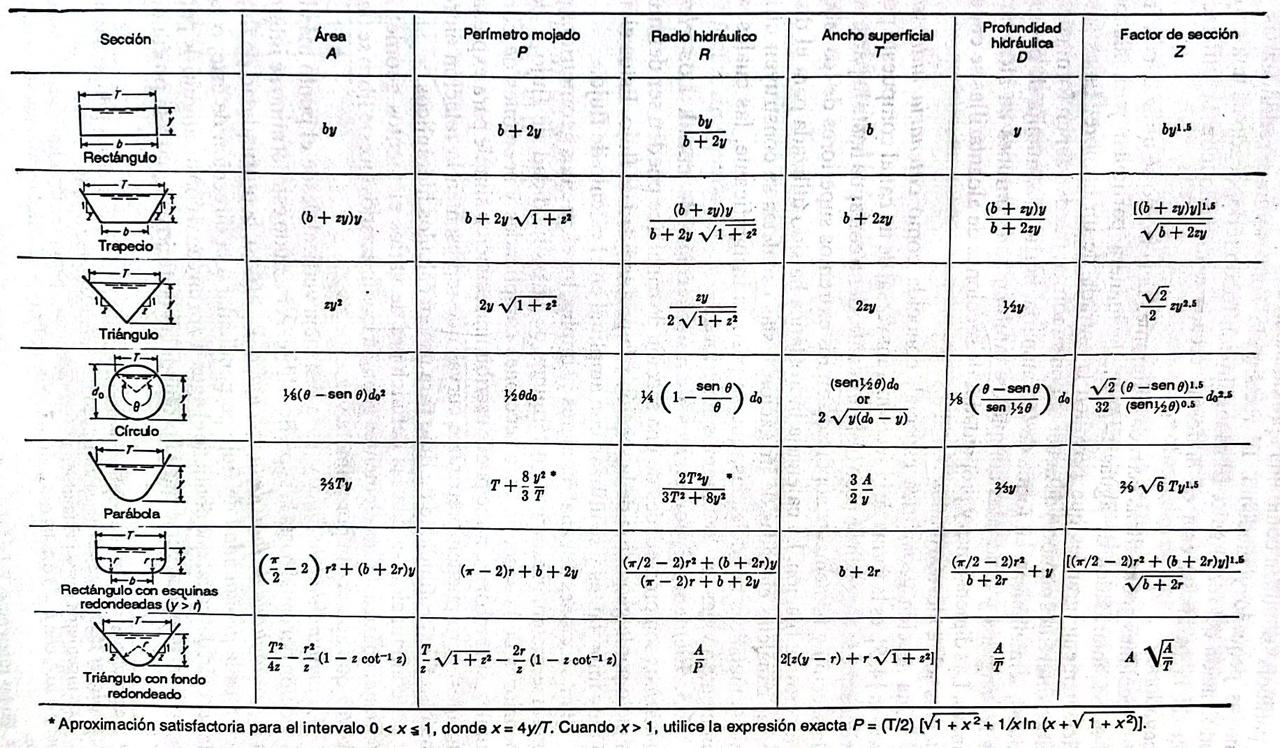
\includegraphics[width=8cm]{fig3.jpeg}
\caption{Perfiles de la lamina de flujo (tomado de \cite{Chau}).}
\label{fig3}
\end{figure}
 
El comportamiento de los  perfiles de lamina de agua se puede hacer con base en el analysis de la ecuaci\'on~\ref{eq5}. De acuerdo con esto, $y$ aumentar\'a a lo largo de $x$ si $\frac{dy}{dx}$ es positivo y decrecer\'a si ocurre lo contrario. El signo de $\frac{dy}{dx}$ lo determina la parte derecha de la ecuaci\'on~\ref{eq5}; los signos del numerador ($S_o - S_f $) y del denominador ($1-F_r^2$). Del estudio de flujo uniformes sabemos que $S_f = S_o = S_w$ cuando $y_n = y$, por lo que para un $Q$ dado a partir de la ecuacion de Manning of Chezy tenemos que $S_f > S_o$ si $y< y_n$ y $S_f < S_o$ si $y > y_n$. De acuerdo con esto, podemos establecer el signo de $S_o - S_f$. El signo de ($1-F_r^2$) se determina si el flujo es subcritico ($F_r < 1$) o supercritico ($F_r > 1$). 

Ahora miremos como la superficie de la lamina de agua se aproxima a la profundidad normal, a la profundidad critica o al fondo del canal. Si $y \rightarrow y_n$ entonce $S_f \rightarrow S_o$ y por lo tanto $\frac{dy}{dx} \rightarrow 0$ a pesar que $Fr \neq 1$ (no flujo critico). Esto significa que el la lamina de agua se aproxima asintoticamente a $NDL$. Por otro lado, si $y \rightarrow y_c$ $F_r \rightarrow 1$ por que el denominador tiende a cero. Esto quiere decir que $\frac{dy}{dx} \rightarrow \infty$ a pesar que $S_f \neq S_o$. Esto significa que la lamina de agua se aproxima a $CDL$ verticalmente. En realidad no se aproxima verticalmente ya que esto no es posible fisicamente, pero si con una pendiente muy alta. A pesar que teoricamente la lamina de agua se aproxima verticalmente esto no es posible ya que las distribuciones de presiones cuando la  lamina de agua se curva fuertemente la presi\'on ya no es hidroestatica por lo tanto la ecuaci\'on~\ref{eq5} se viola.  

Por otro lado, cuando $y \rightarrow \infty$, $V \rightarrow 0$ y por lo tanto $F_r$ y $S_f$ tienden a cero. De la ecuacion~\ref{eq5}, tenemos entonce que $\frac{dy}{dx} \rightarrow S_o$. Teniendo en cuenta que para FGV se asume una pendiente pequeña, tenemos que $\frac{dy}{dx} \approx 0$ por lo que la lamina de agua tiende ser horizontal. 

Analicemos ahora lo que ocurre cuando la lamina de agua se aproxima al fondo del canal (e.g $y \rightarrow$). De la ecuaci\'on de Chezy, tenemos que

$$
S_f = \frac{Q^2}{C^2 A^2 R}
$$

donde $C$ es la constante de Chezy, $R= A/P$ es el radio hidr\'aulico. Note que para un canal rectangular muy ancho de ancho $B$, se tiene que $R \approx y$. Reemplazando en la ecuaci\'on~\ref{eq5}, tenemos que:
$$
\frac{dy}{dx} = \frac{gB \left(S_o C^2 B^2 y^3 - Q^2\right)}{C^2 \left(gBy^3 -\alpha B Q^2\right)}
$$

Teniendo en cuenta que $y\rightarrow 0$ cuando se aproxima al fondo del canal, la ecuaci\'on anterior se comvierte en:
$$
\lim_{y \to 0} \frac{dy}{dx} = \frac{g}{\alpha C^2}
$$
Lo anterior quiere decir que cuando $y \rightarrow 0$, la pendiente de la lamina de agua $dy/dx$ es finita, tiene un valor positivo y es una funci\'on de $C$ y de $\alpha$. Sin embargo, si se usa la ecuaci\'on de Manning en lugar de la ecuacion de Chezy, se tiene the $\frac{dy}{dx} \rightarrow \frac{0}{0} \rightarrow \infty$ si $y \rightarrow 0$.

Con base en lo anterior, analisemos los perfiles de lamina de agua cuando $S_o$ es suave, esto quiere decir que $y_n > y_c$. Si analizamos la profundidad de la lamina de agua en las tres zonas:
\begin{itemize}
    \item Zona 1: $y > y_n > y_c$
    \item Zona 2: $y_n > y > y_c$
    \item Zona 2: $y_n > y_c > y$
\end{itemize}

\subsubsection*{Zona 1 (perfil M1)}
Si $y > y_n$, de la ecuacion de Manning o Chezy, se tiene que $S_f < S_o$ lo que significa que el numerador es positivo  en la ecuaci\'on~\ref{eq5}. Como $y > y_c$, $F_r < 1$ por lo que el denominador de la ecuaci\'on~\ref{eq5} es positivo. Los signos de la ecuacion\ref{eq5} son:
$$
\frac{dy}{dx} = \frac{S_o - S_f}{1-F_r^2} = \frac{+}{+} = +
$$
Lo anterior significa que $y$ se incrementa a lo largo de $x$; crece hacia aguas abajo.  Cuando $y \rightarrow y_n$ asintoticamente en direcci\'on aguas arriba ($S_f \rightarrow S_o$), la superficie del agua tiende a ser horizontal ($\frac{dy}{dx}\rightarrow 0$).  

\subsubsection*{Zona 2 (perfil M2)}
Si $y < y_n$, de la ecuacion de Manning o Chezy, se tiene que $S_f > S_o$. Esto quiere decir que el numerador en la ecuaci\'on~\ref{eq5}, es negativo. El denominador sigue siendo positivo as $F_r < 1$ as $y > y_c$. Los signos de la ecuaci\'on~\ref{eq5} quedan:
$$
\frac{dy}{dx} = \frac{S_o - S_f}{1-F_r^2} = \frac{-}{+} = -
$$
Esto quiere decir que $y$ decrece a lo largo de $x$; hacia aguas abajo en donde $y \rightarrow y_c$ asintoticamente y casi vertical. Hacias aguas arriba, $y \rightarrow y_n$ asintoticamente.

\subsubsection*{Zona 3 (perfil M3)}
Si $y < y_n$, de la ecuci\'on de Manning o de Chezy, se tiene que $S_f > S_o$, lo cual significa que el numerador de la ecuaci\'on~\ref{eq5} es negativo. Como $y < y_c$, $F_r >1$ por lo que el denominador de la ecuaci\'on~\ref{eq5} es negativo. Los signos de la ecuaci\'on~\ref{eq5}, son:
$$
\frac{dy}{dx} = \frac{S_o - S_f}{1-F_r^2} = \frac{-}{-} = +
$$
Esto significa que $y$ incrementa a lo largo de $x$; en direcci\'on aguas abajo. Hacia aguas abajo donde $y \rightarrow y_c$ casi verticalmente, mientras que en direcci\'on aguas arriba cuando $y \rightarrow 0$ la pendiente de lamina de agua es finita y positiva (de acuerdo con la ecuaci\'on de Chezy). 

La figura~\ref{fig4} muestra los perfiles de flujo en situaciones reales.
% Chau fig 5.4
\begin{figure}[h]
\centering
%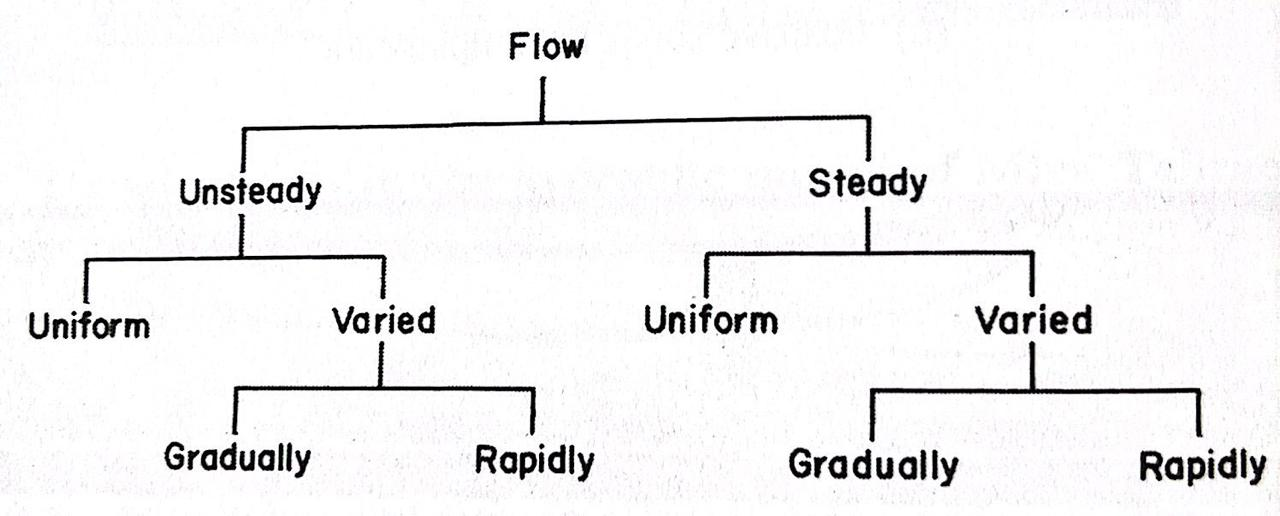
\includegraphics[width=8cm]{fig4.jpeg}
\caption{Perfiles de la lamina de agua (tomado de \cite{Chau}).}
\label{fig4}
\end{figure}

\subsection{Esquematizar los perfiles de flujo}
Es importante anotar que una secci\'on de flujo en donde exista una relacion entre $Q$ y $y$ (e.g. $f(y)=Q$) es una \emph{secci\'on de control}. El comportamiento de los perfiles de flujo analisados son para canales prismaticos con secciones de control aguas arriba o aguas abajo. Sin embargo, en la vida real, los controles sobre el flujo pueden existir en cualquier secci\'on a lo largo del flujo y la geometria asi como la pendiente pueden cambiar a lo largo del canal por lo que la esquematizacion de los perfiles se debe hacer por sectores del canal. A continuacion describe como esquematizar el perfil de flujo en canal:
\begin{enumerate}
    \item Divida el canal en diferentes tramos con una unica geometria, pediente, caudal y coeficiente de friccion.
    \item Cacule la profundidad normal ($y_n$) y la profundidad cr\'itica ($y_c$).
    \item Para cada tramo, dibuje el fondo del canal, la linea de $y_n$ y de $y_c$.
    \item Determine las secciones de control, aquellas secciones en donde $y$ es conocida e.g. secciones en donde $y = y_c$. Indentifique los tramos en donde el flujo es uniforme $y = y_n$.
\end{enumerate}
Note que el flujo subcritico es gobernado por  secciones de control aguas abajo, mientras que el flujo supercritico es cobernado por secciones de control aguas arriba. Es posible tener secciones de control intermedias como vertederos, compuertas, etc, que determinan el flujo aguas arriba y aguas abajo. Por ejemplo, a la entrada de un canal, la profundidad de flujo pasa a travez de $y_c$ cuando el nivel en el tamque o vertedero es mayor que $y_c$ y la pendiente del canal es alta. En un canal que descarga libremente, si $y > y_c$, la lamina de agua pasa por $y_c$ aproximadamente de 3 a 4 veces $y_c$ aguas arriba de la seccion de descarga. Por otra parte, un resalto hidraulico es formado cuando se presenta un cambio de flujo supercritico a subcritico; en este caso se tienen un control aguas arriba y otro aguas abajo del resalto.

% Ej 5.1 Chau 
\begin{eje}{}{eje1}
Esquematice el perfil de flujo de el  canal que conecta los tanques que muestra la figura. Tenga en cuenta que la pendiente del canal 1 es fuerte y la pendiende del canal 2 es suave.
%\centering
%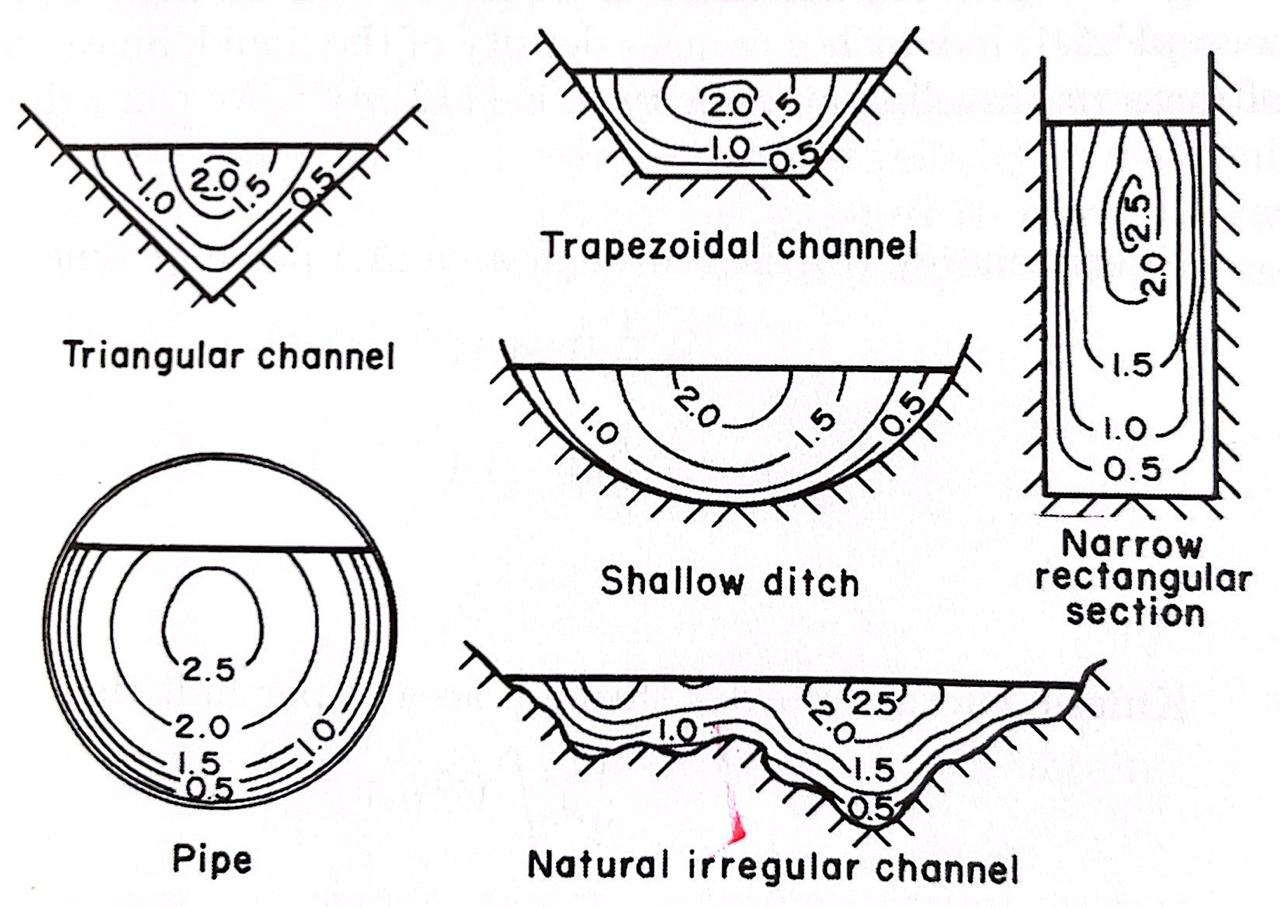
\includegraphics[width=8cm]{fig5.jpeg}
\end{eje}





% REFERENCES
\bibliographystyle{plain} % We choose the "plain" reference style
\bibliography{refs} % Entries are in the refs.bib file

\end{document}
